% !TEX program = xelatex


\documentclass{article} 
\usepackage{xltxtra} % 这个包是为了打印\XeLaTeX 的Logo。 
\usepackage{xeCJK} % 这个包可以指定中文字体。
\setCJKmainfont[Mapping=tex-text,BoldFont=SimHei]{SimSun}
\setCJKsansfont{SimHei}
\setCJKmonofont[Scale=.85]{FandolFang}
\setmainfont{Palatino Linotype}
\setmonofont{Consolas}

\usepackage{url}
\usepackage{geometry}
\geometry{left=3cm,right=3cm}

\usepackage{multirow}
\usepackage{amsfonts}

\newcommand{\e}[1]{$ \times 10^{#1}$}
\renewcommand{\figurename}{图}
\renewcommand{\tablename}{表}
\renewcommand{\today}{\number\year 年 \number\month 月 \number\day 日}

\begin{document}
 \title{Recommder System Handbook学习笔记\ 第一部分,章节4 基于邻域推荐方法的综合调查}
 \author{littlekideee}
 \maketitle

 \section{介绍}
 推荐问题被定义为:基于存于系统中的历史信息,估计一个用户对新产品的反应,并向用户建议那些预测反馈高的新的或老的产品。

 \subsection{问题的一般定义}
 为了给出产品推荐任务的一个一般定义,首先需要介绍一下符号标记。
 \begin{itemize}
 \item $\mathcal{U}$:系统中用户集合。
 \item $\mathcal{I}$:产品集合。
 \item $\mathcal{R}$:评分记录集合。
 \item $\mathcal{S}$:评分可能的值的集合。(例如,$\mathcal{S}=[1,5]$或$\mathcal{S}=\{like,dislike\}$)。
 \item $r_{ui}$:表示用户$u\in \mathcal{U}$对产品$i\in\mathcal{I}$的评分。
 \item $\mathcal{U}_i$:评分过产品$i$的用户子集。
 \item $\mathcal{I}_u$:被用户$u$评分过的产品子集。
 \item $\mathcal{I}_{uv}$:表示同时被用户$u$和$v$评分过的产品集合。
 \item $\mathcal{U}_{ij}$:表示既评分过产品$i$又评分过产品$j$的用户集合。
 \end{itemize}

 推荐系统中两个最重要的问题是best item和top-N推荐问题。第一个问题:对于一个特定的用户$u$,新的项目$i\in\mathcal{I}\backslash\mathcal{I}_u$是$u$最可能感兴趣的那个。当评分是可用的,这个任务通常为定义为一个回归或多类分类问题,目标是学习一个函数$f:\mathcal{U}\times\mathcal{I}\to\mathcal{S}$,它预测一个用户$u$对新项目$i$的评分$f(,u,i)$。这个函数被用来推荐活跃用户$u_a$一个项目$i^*$,这个项目的估计评分是最高的:
 $$ i^*=\mathop{\mathsf{argmax}}\limits_{j\in\mathcal{I}\backslash\mathcal{I}_u}f(u_a,j) $$

 通常评分$\mathcal{R}$被分割为训练集$\mathcal{R}_{train}$学习$f$,和测试集$\mathcal{R}_{test}$来评估预测准确性。两个常用的方法是平均绝对误差(MAE):
 $$ \mathsf{MAE}(f)=\frac{1}{|\mathcal{R}_{test}|}\mathop{\sum}\limits_{r_{ui}\in\mathcal{R}_{test}}|f(u,i)-r_{ui}| $$

 以及根均方差(RMSE):
 $$ \mathsf{RMSE}(f)=\sqrt{\frac{1}{|\mathcal{R}_{test}|}\mathop{\sum}\limits_{r_{ui}\in\mathcal{R}_{test}}(f(u,i)-r_{ui})^2} $$

 如果评分时不可用的,比如只有用户的购买记录,度量评分预测准确度是不可能的。在这种情况下,推荐最好项目的任务就转化为想活跃用户$u_a$推荐一个包含了$N$个项目用户可能感兴趣的列表$L(u_a)$。把项目集合$\mathcal{I}$分成训练集$\mathcal{I}_{train}$,来学习$L$,和测试集$\mathcal{I}_{test}$。令$T(u)\subset{I}_u\cap\subset{I}_{test}$。推荐方法的表现通过精确率和召回率来度量:
 $$ \mathsf{Precision}(L)=\frac{1}{\mathcal{U}}\mathop{\sum}\limits_{u\in\mathcal{U}}|L(u)\cap T(u)|/|L(u)| $$

 $$ \mathsf{Recall}(L)=\frac{1}{\mathcal{U}}\mathop{\sum}\limits_{u\in\mathcal{U}}|L(u)\cap T(u)|/|T(u)| $$

 这个任务的一个缺点是推荐列表$L(u)$中的每一个项目都被认为对用户$u$是同样感兴趣的。一种改进是把列表中的项目通过“兴趣度”排序。如果随机选择测试集,对每个用户$u$,单个项目$i_u\in\mathcal{I}_u$,$L$的效果可以用平均倒数命中率(ARHR)来计算:
 $$ \mathsf{ARHR}(L)=\frac{1}{|\mathcal{U}|}\mathop{\sum}_{u\in\mathcal{U}}\frac{1}{\mathsf{rank}(i_u,L(u))} $$

 其中$\mathsf{rank}(i_u,L(u))$是项目$i_u$在$L(u)$中的位置,如果$i_u\notin L(u)$,则为$\infty$。

 \subsection{推荐方法的概述}
 90年代中期,推荐问题成为一个独立的研究领域。这个问题的解决方法通常分为两类:基于内容和协同过滤方法。

 \subsubsection{基于内容的方法}
 基于内容方法的一般原则是去识别那些有共同特征的项目。在基于内容的推荐系统中,描述每个项目$i$的性质的丰富的信息都被存储在特征向量$\mathbf{x}_i$中。如果项目是文本数据,那么,向量中常包含最富信息的关键词的TF-IDF权重。进一步的,对每一个用户$u$,一个偏好描述向量$\mathbf{x}_u$通常根据项目集合$\mathcal{I}_u$来获得。计算方法是Rocchio算法。这个技术在每当用户对一个产品$i$评分时,就通过在$\mathbf{x}_u$上加$\mathbf{x}_i$更新$\mathbf{x}_u$:
 $$ \mathbf{x}_u=\mathop{\sum}\limits_{i\in\mathcal{I}_u}r_{ui}\mathbf{x}_i $$

 我们可以推荐那些特征向量$\mathbf{x}_i$与描述向量$\mathbf{x}_u$最相似的项目。例如使用余弦相似度来作为最小判别长度(MDL)。这个方法同样可以用来预测评分,为每一个评分值$r\in\mathcal{S}$建立一个内容描述向量$\mathbf{x}_u^{(r)}$作为项目特征向量的平均,这些项目从用户$u$处得到这个评分值。预测评分$\hat{r}_{ui}$就是那个与$\mathbf{x}_u$最相似的$\mathbf{x}_u^{(r)}$中的$r$值。

 基于内容的推荐系统常受限于两个问题:内容分析限制和过度专一化。前者是指内容的数量常常很少。后者是指基于内容的推荐系统常常无法推荐不同类型的项目。

 \subsubsection{协同过滤方法}
 协同过滤方法依赖于用户$u$的评论和系统中其他用户的评分。关键思想是,如果用户$u$和$v$评分的方式相同,那么就把用户$v$喜欢的项目推荐给用户$u$。

 协同过滤方法可以大体被分为两类:邻域方法和基于模型方法。基于邻域(memory-based或heuristic-based)的协同过滤中,系统中存储的用户-项目评分被直接用来预测新项目的评分。具体有两种形式:基于用户和基于项目的推荐。基于用户的系统,通过其他用户(邻居)的评分来评估用户$u$对项目$i$的兴趣。基于项目的方法,则是推荐用户那些与他评分过的项目相似的项目。

 相比于直接把评分拿来预测的基于邻域的系统,基于模型的方法是用这些评分学习一个可预测的模型。大概想法是为系统中的用户和项目建立表示他们潜在属性的特征模型。基于模型的方法有:贝叶斯聚类,潜在语义分析,LDA,最大熵,玻尔兹曼机,SVM和奇异值分解。

 \subsection{邻域方法的优点}
 基于邻域方法的优点主要是:
 \begin{itemize}
 \item 简单:基于邻域的方法是直观而且实施起来相对简单的。在它们最简单的形式下,只需要调节一个参数(邻居的数量)。
 \item 合理性:推荐的理由简单而且直观。
 \item 效率:不像大部分基于模型的系统,基于邻域的在训练阶段花费较少,尽管在推荐阶段需要花费比基于模型更多的资源,但是这是可以先下提前计算的。而且存储这些邻居也只需要花费少量的内存。
 \item 稳定性:当新用户加入系统时,系统是不需要重新训练的。
 \end{itemize}
 
 \section{基于邻域的推荐系统}
 基于邻域的推荐系统的想法是把那些与目标用户想法相近的用户喜爱的项目推荐给他。

 例:如图1所示,用户Eric在考虑是否要租他没看过的电影“Titanic”。他知道Lucy与自己有着非常相近的品位,因为他们都讨厌“The Matrix”,喜欢“Forrest Gump”,因此Eric询问Lucy她对这部电影的看法。另一方面,Eric发现他和Diane品位不同,Diane喜欢动作片而他不喜欢,因此他不会采纳Diane的观点或者采纳Diane相反的观点。

 \begin{figure}[!htb]
	  \begin{center}
	  	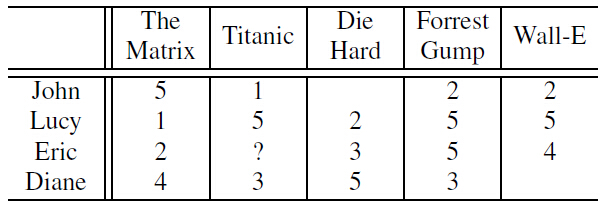
\includegraphics[scale=0.6]{f1.jpg}
	  	\caption{一个基于邻域的例子,显示了4个用户对四部电影的评分}
	  \end{center}
 \end{figure}

 \subsection{基于用户的评分预测}
 基于用户的邻域推荐方法预测一个用户$u$对一个新项目$i$的评分$r_{ui}$通过哪些与$u$最相似(被称为最近邻)的用户对$i$的评分。假设用户$u$与用户$v$之间的相似程度记为$w_{uv}$。$u$的k近邻(k-NN),记为$\mathcal{N}(u)$,是用户$u$$k$个$w_{uv}$最高的用户。我们把$k$个最近邻同时对$i$评分过的用户集合记为$\mathcal{N}_i(u)$。评分$r_{ui}$则使用这些邻居的分数的平均分来估计:
 $$ \hat{r}_{ui}=\frac{1}{|\mathcal{N}_(u)|}\mathop{\sum}\limits_{v\in\mathcal{N}_i(u)}r_{vi} $$

 如果把邻居的相似性权重考虑进来,则预测评分变成加权平均:
 $$ \hat{r}_{ui}=\frac{\mathop{\sum}\limits_{v\in\mathcal{N}_i(u)}w_{uv}r_{vi}}{\mathop{\sum}\limits_{v\in\mathcal{N}_i(u)}|w_{uv}|} $$

 $w_{uv}$可以被替换为$w^{\alpha}_{uv}$,其中$\alpha$是放大因子。通常取$\alpha>1$,使接近$u$的用户具有更大的权重。

 上式还有一个重要的缺陷:它没有考虑到用户对一个项目可能使用不同的评判标准,有的人严格,有的人宽松。解决方法通常是把邻居的评分$r_{vi}$转化成归一化的$h(r_{vi})$,预测分变为:
 $$ \hat{r}_{ui}=h^{-1}\left(\frac{\mathop{\sum}\limits_{v\in\mathcal{N}_i(u)}w_{uv}h(r_{vi})}{\mathop{\sum}\limits_{v\in\mathcal{N}_i(u)}|w_{uv}|}\right) $$

 \subsection{基于用户的分类器}
 以上描述的方法本质是解决了一个回归的问题。基于邻域的分类器,另一方面来说,找到用户$u$对项目$i$最可能的评分,通过$u$的最近邻对这个值进行投票。投票$v_{ir}$:
 $$ v_{ir}=\mathop{\sum}\limits_{v\in\mathcal{N}_i(u)}\delta(r_{vi}=r)w_{uv} $$

 其中,如果$r_{vi}=r$,则$\delta(r_{vi}=r)$为1,反之,为0。预测评分是那个使$v_{ir}$最大的评分$r$。

 分类方法也能考虑定义归一化的评分。令$\mathcal{S}^{'}$为可能的归一化的值的集合(可能需要时离散的),预测评分为:
 $$ \hat{r}_{ui}=h^{-1}\left(\mathop{\mathsf{argmax}}\limits_{r\in\mathcal{S}^{'}}\mathop{\sum}\limits_{v\in\mathcal{N}_i(u)}\delta(h(r_{vi})=r)w_{uv}\right) $$

 \subsection{回归VS分类}
 选择基于邻域的回归还是分类方法很大程度上取决于系统的评分粒度。如果评分是连续的,那么使用回归方法更加适合。相反,如果评分时粒度是少数几个离散值时,或评分值不能按照一个明显的方式排列,则使用分类方法较好。另外,由于归一化会趋向于把评分映射到一个连续的粒度上,分类方法就变得难以处理了。

 \subsection{基于项目的推荐系统}
 基于项目的方法关注于给予相似项目的评分。

 记$\mathcal{N}_u(i)$为与用户$u$评分的过的项目$i$相似的项目集合。则$u$对$i$的预测评分为:
 $$ \hat{r}_{ui}=\frac{\mathop{\sum}\limits_{j\in\mathcal{N}_u(i)}w_{ij}r_{uj}}{\mathop{\sum}\limits_{j\in\mathcal{N}_u(i)}|w_{ij}|} $$

 同样的,用户个人评分粒度的区别也能使用归一化评分$h$处理:
 $$ \hat{r}_{ui}=h^{-1}\left(\frac{\mathop{\sum}\limits_{j\in\mathcal{N}_u(i)}w_{ij}h(r_{uj})}{\mathop{\sum}\limits_{j\in\mathcal{N}_u(i)}|w_{ij}|}\right) $$

 而且,我们同样可以定义一个基于项目的分类方法:
 $$ \hat{r}_{ui}=h^{-1}\left(\mathop{\mathsf{argmax}}\limits_{r\in\mathcal{S}^{'}}\mathop{\sum}\limits_{j\in\mathcal{N}_u(i)}\delta(h(r_{uj})=r)w_{ij}\right) $$

 \subsection{基于用户VS基于项目推荐系统}
 5个选择基于用户还是基于项目的方法的评判标准:
 \begin{itemize}
 \item 准确率:基于邻域的推荐方法大部分取决于用户和项目数量的比率。在基于用户方法中决定一个用户邻居的相似性通常通过比较这些用户在同一个项目上的评分获得。考虑一个10000评分,1000用户,100个项目的系统,同时假设评分在项目之上是分布均匀的。由表1,用户可作为潜在邻居的平均数在650。然而用于计算相似度的公共评分的平均数量只有1。另一方面,一个基于项目的方法通常通过比较相同用户对这些项目的评分来计算两个项目的相似度。这时,我们发现现在邻居的平均数量在99,用户计算相似度的评分平均数量为10。
 \begin{table}[!htb]
 \centering
 \caption{在基于用户和基于项目方法中用于计算相似度的平均邻居数量和平均评分数量。评分均匀分布假设每个用户的评分数量为$p=|\mathcal{R}|/|\mathcal{U}|$,每个项目的评分数量为$q=|\mathcal{R}|/|\mathcal{I}|$}
 	\begin{tabular}{c||c|c} \hline
 	           & Avg.neighbors & Avg.ratings \\ \hline
 	User-based & $(|\mathcal{U}|-1)\left(1-\left(\frac{|\mathcal{I}|-p}{\mathcal{I}}\right)^p\right)$ & $\frac{p^2}{|\mathcal{I}|}$ \\ \hline
 	Item-based & $(|\mathcal{I}|-1)\left(1-\left(\frac{|\mathcal{U}|-q}{\mathcal{U}}\right)^q\right)$ & $\frac{q^2}{|\mathcal{U}|}$ \\ \hline
 	\end{tabular}
 \end{table}

 当用户数远远大于项目数时,基于项目的方法会产生更加准确的推荐。相反的话,基于用户的方法更好。

 \item 效率:如表2所示,推荐系统的内存和计算效率同样依赖于用户和项目数量的比率。因此,当用户数量大于项目时,基于项目的方法需要使用的内存和计算相似度的计算量(训练阶段)都小于基于用户的方法。然而在线推荐阶段的时间复杂度上两个方法是相同的,因为它仅依赖于可用项目的数量和邻居的最大值。
 \begin{table}
 \centering
 \caption{基于用户和基于项目的邻域方法需要的空间和时间复杂度,$p=\mathsf{max}_u|\mathcal{I}_u|$,$q=\mathsf{max}_i|\mathcal{U}_i|$,邻域中邻居最大值为$k$}
 \begin{tabular}{c||c|c|c}\hline
 \multirow{2}*{\ } & \multirow{2}*{Space} & \multicolumn{2}{c}{Time} \\ 
                   &                      & Training  & Online \\ \hline
 User-based        & $O(|\mathcal{U}|^2)$ & $O(|\mathcal{U}|^2p)$ & $O(|\mathcal{I}|k)$ \\
 Item-based        & $O(|\mathcal{I}|^2)$ & $O(|\mathcal{I}|^2q)$ & $O(|\mathcal{I}|k)$ \\ \hline
 \end{tabular}
 \end{table}
 \item 稳定性:选择基于用户还是基于项目的方法还依赖于系统中用户或者项目数量的变化和变化的频率。如果项目数量较稳定的话,选用基于项目的方法较好,反之亦然。
 \item 合理性:基于项目的方法很容易解释推荐。而基于用户的方法就不适合,因为用户不认识这些“邻居”。
 \item 意外发现率(长尾发现能力):基于项目的方法一般推荐的都是用户所喜欢的项目类似的项目,因此很难发现那些不同类型的项目。然而,由于使用用户相似度,基于用户的方法更可能做出意外发现的推荐。
 \end{itemize}

 \section{邻域方法的构成}
 除了上述的那些属性之外。邻域推荐系统好友三个重要的点:1)评分的归一化,2)相似度权重的计算,3)邻居的选择。

 \subsection{评分归一化}
 当用户评分一个项目的时候,每个用户都有自己个人的尺度,因此,我们要对他们的评分进行归一化处理。把个人评分转化成更一般的尺度的两种最流行的评分归一化模式是mean-centering和Z-score。
 \subsubsection{Mean-centering}
 Mean-centering的想法是不管评分正负都和均值作比较。在基于用户的推荐中,一个原始评分$r_{ui}$转化到均值中心是通过减去均值$\bar{r}_u$得到:
 $$ h(r_{ui})=r_{ui}-\bar{r}_u $$

 则预测评分就可以写为:
 $$ \hat{r}_{ui}=\bar{r}_u+\frac{\mathop{\sum}\limits_{v\in\mathcal{N}_i(u)}w_{uv}(r_{vi}-\bar{r}_{v})}{\mathop{\sum}\limits_{v\in\mathcal{N}_i(u)}|w_{uv}|} $$

 基于项目的均值中心归一化:
 $$ h(r_{ui})=r_{ui}-\bar{r}_i $$

 预测评分为:
 $$ \hat{r}_{ui}=\bar{r}_i+\frac{\mathop{\sum}\limits_{j\in\mathcal{N}_u(i)}w_{ij}(r_{uj}-\bar{r}_j)}{\mathop{\sum}\limits_{j\in\mathcal{N}_u(i)}|w_{ij}|} $$
 
 \subsubsection{Z-score归一化}
 考虑这样一种情况:用户$A$和$B$的平均分都是3。但$A$的评分在1到5分之间都有,$B$则都是3分,那么如果他们给一个项目评了5分,则反映$B$对这个项目有更大的欣赏。Mean-centering移除了偏移量,而Z-score把在个人评分尺度中传播的东西也考虑在内。

 在基于用户的方法中,评分的归一化是在均值中心方法的基础上在除以一个标准差:
 $$ h(r_{ui})=\frac{r_{ui}-\bar{r}_u}{\sigma_u} $$

 预测分就变成了:
 $$ \hat{r}_{ui}=\bar{r}_u+\sigma_u\frac{\mathop{\sum}\limits_{v\in\mathcal{N}_i(u)}w_{uv}(r_{vi}-\bar{r}_{v})/\sigma_v}{\mathop{\sum}\limits_{v\in\mathcal{N}_i(u)}|w_{uv}|} $$

 类似的,基于项目的方法Z-score归一化为:
 $$ h(r_{ui})=\frac{r_{ui}-\bar{r}_i}{\sigma_i} $$

 预测分为:
 $$ \hat{r}_{ui}=\bar{r}_i+\sigma_i\frac{\mathop{\sum}\limits_{j\in\mathcal{N}_u(i)}w_{ij}(r_{uj}-\bar{r}_j)/\sigma_j}{\mathop{\sum}\limits_{j\in\mathcal{N}_u(i)}|w_{ij}|} $$

 \subsubsection{选择归一化方法}
 在某些情况下,评分归一化会产生不良的影响。例如,一个用户给他购买过的项目都打了最高的评分,Mean-centering方法认为之歌用户是“容易取悦的”,任何评分低于这个最高分都被人为是负面评分。然而,这个用户可能是一个“不易取悦的”用户,他会仔细考虑选择那很确定会喜欢的项目。进一步地,在很少的评分上归一化会产生难以预期的结果。例如,用户的评分很少,那么标准差就会是0,那么预测评分就没有意义了。尽管如此,在评分数据不是很稀疏时,归一化策略对预测还是有很大帮助的。

 对比Mean-centering和Z-score,后者的优势是考虑了个体用户或项目的评分变化。当评分粒度是大范围离散值或连续值时,这个方法十分有用。但由于评分被除以或乘以一个标准差,Z-score比Mean-centering更加敏感,预测的评分通常在评分刻度之外。

 最后,如果评分归一化没有提升结果,其他的方法可以采用基于偏好的过滤方法。

 \subsection{相似性权重计算}
 相似度权重在基于邻域的推荐方法中有着双重作用:1)它们可以用于选择信任领域,2)它们提供在预测中给予这些邻居多少重要性的依据。

 \subsubsection{基于关联的相似性}
 在信息检索领域常用的一种度量相似性的方法是为两个向量$\mathbf{x}_a$和$\mathbf{x}_b$计算余弦向量相似度(Cosine Vector(CV)):
 $$ \mathsf{cos}(\mathbf{x}_a,\mathbf{x}_b)=\frac{\mathbf{x}_a^{\top}\mathbf{x}_b}{\|\mathbf{x}_a\|\|\mathbf{x}_b\|} $$

 在项目的推荐中,把一个用户$u$看做一个向量$\mathbf{x}\in\mathbb{R}^{|I|}$,其中如果用户$u$对项目$i$产生过评分,则$\mathbf{x}_{ui}=r_{ui}$,反之为0。用户$u$和$v$的相似度为:
 $$ CV(u,v)=\mathsf{cos}(\mathbf{x}_{u},\mathbf{x}_{v})=\frac{\mathop{\sum}\limits_{i\in\mathcal{I}_{uv}}r_{ui}r_{vi}}{\sqrt{\mathop{\sum}\limits_{i\in\mathcal{I}_{u}}r_{ui}^2\mathop{\sum}\limits_{j\in\mathcal{I}_{v}}r_{vj}^2}} $$

 这个度量方法的一个问题是没有考虑到均值的差异和两个用户评分的方差。

 一个更加流行的比较评分的方法是Pearson相关系数(PC):
 $$ PC(u,v)=\frac{\mathop{\sum}\limits_{i\in\mathcal{I}_{uv}}(r_{ui}-\bar{r}_{u})(r_{vi}-\bar{r}_{v})}{\sqrt{\mathop{\sum}\limits_{i\in\mathcal{I}_{uv}}(r_{ui}-\bar{r}_{u})^2\mathop{\sum}\limits_{i\in\mathcal{I}_{uv}}(r_{vi}-\bar{r}_{v})^2}} $$

 同样地,计算两个项目的相似度为:
 $$ PC(i,j)=\frac{\mathop{\sum}\limits_{u\in\mathcal{U}_{ij}}(r_{ui}-\bar{r}_{i})(r_{uj}-\bar{r}_{j})}{\sqrt{\mathop{\sum}\limits_{u\in\mathcal{U}_{ij}}(r_{ui}-\bar{r}_{i})^2\mathop{\sum}\limits_{u\in\mathcal{U}_{ij}}(r_{uj}-\bar{r}_{j})^2}} $$

 用户评分尺度的不同作用是大于项目评分的不同的。因此在计算相似度的时候把均值换成用户的评分均值,调整的余弦(AC)相似度为:
 $$ AC(i,j)=\frac{\mathop{\sum}\limits_{u\in\mathcal{U}_{ij}}(r_{ui}-\bar{r}_{u})(r_{uj}-\bar{r}_{u})}{\sqrt{\mathop{\sum}\limits_{u\in\mathcal{U}_{ij}}(r_{ui}-\bar{r}_{u})^2\mathop{\sum}\limits_{u\in\mathcal{U}_{ij}}(r_{uj}-\bar{r}_{u})^2}} $$

 在某些情况下AC相似度比PC相似度表现的更好。

 \subsubsection{其他的相似度度量方法}
 \begin{itemize}
 \item 平均平方差异(MSD)
 $$ MSD(u,v)=\frac{|\mathcal{I}_{uv}|}{\mathop{\sum}\limits_{i\in\mathcal{I}_{uv}}(r_{ui}-r_{vi})^2} $$

 它表现比PC相似度差,因为它没有考虑到用户偏好或产品的被欣赏程度之间的负相关。

 \item 斯皮尔曼等级相关(SRC)
 PC直接使用评分的值,SRC使用这些评分的等级。用$k_{ui}$来表示用户$u$评分列表中项目$i$的等级,则两个用户的SRC相似度为:
 $$ SRC(u,v)=\frac{\mathop{\sum}\limits_{i\in\mathcal{I}_{uv}}(k_{ui}-\bar{k}_{u})(k_{vi}-\bar{k}_{v})}{\sqrt{\mathop{\sum}\limits_{i\in\mathcal{I}_{uv}}(k_{ui}-\bar{k}_{u})^2\mathop{\sum}\limits_{i\in\mathcal{I}_{uv}}(k_{vi}-\bar{k}_{v})^2}} $$

 SRC的主要优点是它避免了评分归一化的问题,但当评分只有几个值时,它不是一个好方法。由于需要排序,它的计算量也打很多。
 \end{itemize}

 表3是使用MSD,SRC和PC三种相似度方法在MovieLens数据集上的MAE实验结果。
 \begin{table}[!htb]
 	\centering
 	\caption{分别使用MSD,SRC,PC的MAE实验结果。使用邻居数量$k$}
 	\begin{tabular}{c||c|c|c}\hline
 	k  &   MSD  & SRC & PC \\ \hline\hline
 	5 & 0.7898 & 0.7855 & 0.7829\\ \hline
 	10 & 0.7718 & 0.7636 & 0.7618\\ \hline
 	20 & 0.7634 & 0.7558 & 0.7545\\ \hline
 	60 & 0.7602 & 0.7529 & 0.7518\\ \hline
 	80 & 0.7605 & 0.7531 & 0.7523\\ \hline
 	100 & 0.7610 & 0.7533 & 0.7528\\ \hline
 	\end{tabular}
 \end{table}

 \subsubsection{重要性考量}
 由于用户评分矩阵的稀疏,在计算相似度时,如果可用来计算的评分数量很少,那么计算的结果就不能真实反映两个用户或项目之间的相似度。

 将相似度权重的重要性考虑在内的一些策略主要想法是降低那些仅使用很少一部分评分计算相似度的权重。例如在Significant加权中,如果两个用户共同评分的项目数少于阈值$\gamma$,那么一个用户相似度权重$w_{uv}$需要乘以一个惩罚项:
 $$ w_{uv}^{'}=\frac{\mathsf{min}\{|\mathcal{I}_{uv},\gamma|\}}{\gamma}\times w_{uv} $$

 同样地,项目相似度变为:
 $$ w_{ij}^{'}=\frac{\mathsf{min}\{|\mathcal{U}_{ij},\gamma|\}}{\gamma}\times w_{ij} $$

 有文献之处,当$\gamma\geq 25$时,预测评分的准确率会提高,而当这个值为50时,结果最好。

 还有一种方法是基于“收缩”的概念:
 $$ w_{uv}^{'}=\frac{|\mathcal{I}_{uv}|}{|\mathcal{I}_{uv}|+\beta}\times w_{uv} $$

 $$ w_{ij}^{'}=\frac{|\mathcal{U}_{ij}|}{|\mathcal{U}_{ij}|+\beta}\times w_{ij} $$ 

 \subsubsection{方差考量}
 用户评分的方差蕴含着这个用户评分给我们的信息,如果一个用户总是评最高分,那么他的评分参考意义就不是很大。

 一个解决这个问题方法是逆用户频率,它基于信息检索中的逆文档频率(IDF),给每个项目$i$一个权重$\lambda_{i}$:
 $$ \lambda_i=\mathsf{log}\frac{|\mathcal{U}|}{|\mathcal{U}_i|} $$

 然后我们可以计算一个频率加权皮尔逊相关系数(FWPC):
 $$ FWPC(u,v)=\frac{\mathop{\sum}\limits_{i\in\mathcal{I}_{uv}}\lambda_i(r_{ui}-\bar{r}_{u})(r_{vi}-\bar{r}_{v})}{\sqrt{\mathop{\sum}\limits_{i\in\mathcal{I}_{uv}}\lambda_i(r_{ui}-\bar{r}_{u})^2\mathop{\sum}\limits_{i\in\mathcal{I}_{uv}}\lambda_i(r_{vi}-\bar{r}_{v})^2}} $$

 除此之外,还有一些其他的方法,比如通过最大或用户间的平均相似度来计算因子$\lambda_i$。再给出一个项目加权向量$\lambda=(\lambda_1,\dots,\lambda_{|\mathcal{I}|})$,用户之间的相似度可由$u$可能与$v$具有相同评分行为的似然来计算:
 $$ \mathsf{Pr}(u|v,\lambda)=\frac{1}{Z_{v}}\mathsf{exp}\left(\mathop{\sum}\limits_{i\in\mathcal{I}_{uv}}\lambda_ir_{ui}r_{vi}\right) $$

 其中,$Z_v$是归一化常数。

 \subsection{邻域选择}
 最近邻的数量和选择标准对推荐系统的质量也有影响。最近邻的选择通常分为两步完成:1)一个全局过滤步骤:仅最可能的候选邻居被保留,2)一个预测步骤:在预测是选择最好的候选邻居。

 \subsubsection{邻居的提前过滤}
 提前过滤邻居是一个必须的步骤,他通过减少相似度权重的数量和限制候选邻居的数量来是基于邻域的方法在实践中可行。几个可用的方式:
 \begin{itemize}
 \item Top-N过滤:对每个用户或项目,仅保留最相近的$N$个用户或项目和他们的权重。$N$的取值不宜过大和过小。
 \item 阈值过滤:保留那些权重大于一个给定阈值$w_{min}$的那些最近邻。因为更有意义的邻居被保留下来,这种方法比Top-N更加灵活,但好的$w_{min}$却很难决定。
 \item 负值过滤:一般而言,负关联没有正关联可靠。有实验也证明负关联对预测准确率没有提高。
 \end{itemize}

 注意到这三个方法是可以关联起来满足推荐系统的需求的。

 \subsubsection{预测阶段的邻居}
 在预测新的评分时,使用的是k近邻,即选择相似度最高的k个邻居。关键问题是k如何取值。

 如表3所示,预测准确度随$k$的增加符合一个凹函数。当$k$值较小(如$k<20$)时,预测准确度很低,随着$k$值增大,准确度上升,当$k$大到一定值时,准确度又开始回落。文献中指出,邻居数量在20到50之间较好。最优的$k$值应由交叉验证获得。

 \section{高级技术}
 邻域方法基于评分关联,如之前提到的那些,他们有两个重要的缺陷:
 \begin{itemize}
 \item 覆盖范围限制:因为评分关联通过比较两个用户共同评分过的项目的评分来计算他们的相似度,用户仅当他们有共同评分过的项目才可能成为邻居。这个假设有很大的限制,因为用户评分很少或没有共同评分时,他们仍然有有共同偏好的可能。进一步的,由于只有邻域的项目才会被推荐,方法的覆盖范围也被限制了
 \item 对稀疏数据十分敏感:另一个评分关联的问题是可用评分数据的缺少。冷启动问题是这类问题的一个极端情况。当评分数据稀疏的时候,两个用户或项目之间的共同评分数量非常少,基于邻域的方法则会受制于邻域的大小。
 \end{itemize}

 一个解决这些问题的通用方法是给缺失评分填上默认值,如评分范围的中间值或用户项目评分的均值。更可靠的方法是使用内容信息去填写缺失评分。缺失评分可由基于内容的方法来代替预测。内容的相似度可以用来代替或添加的评分关联相似度。

 然而这些方法仍有缺点,接下来介绍两种解决覆盖率和稀疏度的方法:降维和基于图的方法。

 \subsection{维度归约方法}
 维度归约方法把用户或项目投射到一个低维的潜在空间中,这个空间能捕捉他们的重要特征。

 本质上用于推荐系统的维度归约有两种方式:1)用户-项目评分矩阵归约,2)稀疏的相似度矩阵归约。

 \subsubsection{评分矩阵归约}
 项目推荐中一个流行的维度归约方法是潜在语义索引(LSI)。大小为$|\mathcal{U}|\times|\mathcal{I}|$,秩为$n$的用户-项目评分矩阵$R$近似等于矩阵$\hat{R}=PQ^{\top}$,其秩为$k<n$,其中$P$是一个$|\mathcal{U}|\times k$的用户特征矩阵,$Q$是一个$|\mathcal{I}|\times k$的项目特征矩阵。直观上来说,$P$的第$u$行$\mathbf{p}_u\in\mathbb{R}^k$,代表用户$u$投影到$k$维潜在空间的坐标。$Q$的第$i$行$\mathbf{q}_i\in\mathbb{R}^k$,代表项目$i$投影到$k$维潜在空间的坐标。矩阵$P$和$Q$通常由最小化误差得到:
 $$  \mathsf{err}(P,Q)=\|R-PQ^{\top}\|^2_F=\mathop{\sum}\limits_{u,i}(r_{ui}-\mathbf{p}_u\mathbf{q}_i^{\top})^2 $$

 最小化这个误差等价于找到矩阵$R$的一个奇异值分解(SVD):
 $$ R=U\Sigma V^{\top} $$

 其中$U$是一个$|\mathcal{U}|\times n$的矩阵,$V$是一个$|\mathcal{I}|\times n$的矩阵,$\Sigma$是一个$n\times n$的奇异值矩阵。记$\Sigma_k$,$U_k$,$V_k$是选择最大的$k$个奇异值获得的子集。用户和项目的特征矩阵对应为$P=U_k\Sigma_k^{1/2}$和$Q=V_k\Sigma_k^{1/2}$。

 一旦获得了$P$和$Q$,典型的基于模型的评分预测$r_{ui}$为:
 $$ r_{ui}=\mathbf{p}_u\mathbf{q}_i^{\top} $$

 把SVD应用到评分矩阵$R$上的一个主要问题是:大多数$R$中的评分是未定义的。如果填上默认值,数据就会产生偏差,而且矩阵$R$的密度将变得很大。通常的解决方式是只使用已知的评分来学习$P$和$Q$:
 $$ \mathsf{err}(P,Q)=\mathop{\sum}\limits_{r_{ui}\in\mathcal{R}}(r_{ui}-\mathbf{p}_u\mathbf{q}_i^{\top})^2+\lambda(\|\mathbf{p}_u\|^2+\|\mathbf{q}_i\|^2) $$

 其中$\lambda$是控制正则项等级的参数。第五章会详细介绍这种推荐方法。

 在基于邻域的推荐系统中,共同的原则是在潜在空间中计算用户或项目之间的相似度。这可以通过解决一下问题来完成:
 \[
 \begin{array}{l}
 \mathsf{err}(P,Q)=\mathop{\sum}\limits_{r_{ui}\in\mathcal{R}}(z_{ui}-\mathbf{p}_u\mathbf{q}_i^{\top})^2 \\
 \mathsf{subject\ to:}\\
 \|\mathbf{p}_u\|=1,\forall u\in\mathcal{U},\|\mathbf{q}_i\|=1,\forall i\in\mathcal{I}
 \end{array}
 \]

 其中$z_{ui}$是均值中心评分$r_{ui}$归一化到$[-1,1]$区间:
 $$ z_{ui}=\frac{r_{ui}-\bar{r}_u}{r_{max}-r_{min}} $$

 这个问题对应于,在一个k维的球面上,如果两个用户$u$和$v$距离相近,那么他们对相同的项目评分也是相近的,因此两个用户的相似度可以这样计算:
 $$ w_{uv}=\mathbf{p}_u\mathbf{p}_v^{\top} $$

 同样地,两个项目的相似度为:
 $$ w_{ij}=\mathbf{q}_i\mathbf{q}_j^{\top} $$

 \subsubsection{相似度矩阵的归约}
 原则与上节是一样的,把矩阵映射到表示用户和项目主要特征的低维潜在空间中。令$W$为表示用户或项目相似度秩为$n$的对称矩阵。同样的想法,我们希望把$W$近似为一个矩阵$\hat{W}=PP^{\top}$,它的秩$k<n$,并通过最小化一下误差得到:
 $$ \mathsf{err}(P)=\|R-PP^{\top}\|^2_F=\mathop{\sum}\limits_{u,v}(w_{uv}-\mathbf{p}_u\mathbf{p}_v^{\top})^2 $$

 计算特征矩阵$P$等价于计算$W$的特征值分解:
 $$ W=V\Lambda V^{\top} $$

 其中$\Lambda$是一个包含了$W |\mathcal{U}|$个特征值的对角阵。$V$是对应特征向量的$|\mathcal{U}|\times|\mathcal{U}|$的正交阵。令$V_k$是取前$k$个主要特征向量的矩阵。那么,用户的相似度矩阵可以近似为:
 $$ W^{'}=PP^{\top}=V_k\Lambda_kV_k^{\top} $$

 \subsection{基于图的方法}
 在基于图的方法中,数据被表示成图的形式,节点是用户、项目,边代表用户、项目之间的相互关系或相似度。例如图2建立了一个二部图,左边节点是用户,右边节点是电影,边代表用户对电影有过评分,边的权重表示评分。当然,除此之外还有另外一些表示方法。
 \begin{figure}[!htb]
	  \begin{center}
	  	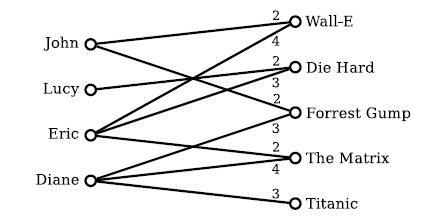
\includegraphics[scale=0.6]{f2.jpg}
	  	\caption{图1的二部图表示法}
	  \end{center}
 \end{figure}

 在这些模型中,标准的基于关联预测方法仅使用那些直接连接的点。而在基于图的方法中,允许节点不直接连接,利用通过边传递信息来表达互相关系的节点。边的权重越大,允许传递的信息就越多。如果两个节点离得很远,那么节点之间影响就很小。这两个属性被称为传播(propagation)和衰减(attenuation)。

 基于图的方法被用于推荐项目有两种方法,第一种是推荐给用户的项目必然在图中离用户“很近”。第二种是图中节点之间的接近程度可以被用来刻画基于邻域方法中的相似度。

 \subsubsection{基于路径的相似度}
 在基于路径的相似度中,两个阶段的距离是他们之间路径的长度的函数。
 \paragraph{最短路径}

 在这个方法中,数据被建模为一个有向图,节点代表用户,边是否存在基于horting和predictability的概念。Horting是在两个用户之间的不对称关联,如果这些用户评分了相似的项目,这种关联就成立。形式化地,一个用户$u$\ horts另一个用户$v$说明$|\mathcal{I}_{uv}\geq\alpha|$和$|\mathcal{I}_{uv}|/|\mathcal{I}_{u}|\geq\beta$同时被满足,其中$\alpha$和$\beta$是先决阈值。另一方面,Predictability属性是指,映射到代表用户$u$和$v$的相同评分尺度下,$u$的评分与$v$的评分相近。因此,$v$可预测$u$,要使$u$\ horts\ $v$,且存在一个线性转换$l:\mathcal{S}\rightarrow\mathcal{S}$如:
 $$ \frac{1}{|\mathcal{I}_{uv}|}\mathop{\sum}\limits_{i\in\mathcal{I}_{uv}}|r_{ui}-l(r_{vi})|\leq\gamma $$

 其中$\gamma$是另一个给定的阈值。

 Predictability在图中被表示成两个节点间的有向边。那么给用户$u$推荐新项目,则转化成在有向图中找到一条$u$到其他用户的最短路径。令$P=\{u,v_1,v_2,\dots,v_m\}$为最短路径,其中$v_m\in\mathcal{U}_i$。$v_m$对项目$i$的评分被一个线性映射的组合转换到用户$u$的评分尺度上:
 $$ \hat{r}_{ui}^{(P)}=(l_m\circ\dots\circ l_2\circ l_1)(r_{vi}) $$

 最终的预测分$r_{ui}$取所有最短路径得到的预测分的平均分得到。

 \paragraph{路径数量}

 二部图中一个用户和一个项目的路径数量可以被用来评估他们的兼容性(compatibility)。令$R$为$|U|\times|I|$的评分矩阵,$r_{ui}$等于1表示用户$u$对项目$i$有评分,反之为0。二部图的邻接矩阵$A$可以定义为:
 \[ 
 A=\left(
 \begin{array}{cc}
 0 & R^{\top}\\
 R & 0
 \end{array}
 \right) 
 \]

 在这个方法中,用户$u$和项目$i$之间的关联被定义为长度不大于给定最大值$K$的所有路径权重之和。为了减少长路径的贡献,长度为$k$的路径权重定义为$\alpha^k$,其中$\alpha\in[0,1]$。节点对之前$k$长路径的数量有$A^k$给出,用户-项目关联矩阵$S_K$为:
 \[
 \begin{array}{lll}
 S_K & = & \mathop{\sum}\limits_{k=1}^K\alpha^kA^k\\
     & = & (I-\alpha A)^{-1}(\alpha A-\alpha^KA^K)
 \end{array}
 \]

 这个计算图中节点间距离的方法被称为Katz量,这个度量和Von Neumann Diffusion kernel很相近:
 $$ K_{VND}=\mathop{\sum}\limits_{k=1}^{\infty}\alpha^kA^k=(I-\alpha A)^{-1} $$

 以及Exponential Diffusion kernel:
 $$ K_{ED}=\mathop{\sum}\limits_{k=1}^{\infty}\frac{1}{k!}\alpha^kA^k=\mathsf{exp}(\alpha A) $$

 其中$A^0=I$。

 \subsubsection{随机游走相似度}
 基于图方法中的传递关联也能用概率框架来定义。在此框架中,用户或项目的相似度通过随机游走到这些节点的概率得到。它可以形式化描述为一个一阶马尔科夫过程,$n$个状态,$n\times n$的概率转换矩阵$P$,在任意时间点$t$,有状态$i$到$j$的概率为:
 $$ p_{ij}=\mathsf{Pr}(s(t+1)=j|s(t)=i) $$

 记$\pi(t)$第$t$步的概率分布向量,即$\pi_i(t)=\mathsf{Pr}(s(t)=i)$,马尔科夫链演变的特点是:
 $$ \pi(t+1)=P^{\top}\pi(t) $$

 这个过程会收敛到一个稳定的分布向量$\pi(\infty)$。

 \paragraph{项目评级}
 与网页评级相似的一个推荐算法是项目评级。这个方法想用户$u$对新项目的偏好评级为图中的随机游走的概率。边的权重由$|\mathcal{I}|\times|\mathcal{I}|$的概率转移矩阵$P$给出,其中$p_{ij}=|\mathcal{U}_{ij}|/|\mathcal{U}|_i$是一个在已知用户评分过项目$i$的条件下用户评分项目$j$的条件概率。

 和页面评级一样,在任意时间$t$,随机游走既可以利用$P$,以固定概率$\alpha$到达邻接节点,又可以以概率$(1-\alpha)$“瞬移”到任意节点。令$\mathbf{r}_u$为评分矩阵$R$的第$u$行,用户$u$“瞬移”到其他节点的概率分布有向量$\mathbf{d}_u=\mathbf{r}_u/\|\mathbf{r}_u\|$给出。则用户$u$在第$t+1$步的状态概率向量可递归的表达为:
 $$ \pi_u(t+1)=\alpha P^{\top}\pi_u(t)+(1-\alpha)\mathbf{d}_u $$

 实践中,$\pi_u(\infty)$通常由初始化为均匀分布(即,$\pi_u(0)=\frac{1}{n}\mathbf{1}_n$)的过程获得,然后通过上式迭代更新$\pi_u$直至收敛。一旦$\pi_u(\infty)$计算完成,系统就可以将$\pi_{ui}$最高的项目$i$推荐给用户$u$了。

 \paragraph{平均首次通过/通勤时间}
 基于随机游走的其他距离度量有平均首次通过时间和平均首次通勤时间。平均首次通过时间$m(j|i)$是随机游走中首次到达节点$j$的平均步骤数。令$P$为$n\times n$的概率转移矩阵,$m(j|i)$可递归得到:
 \[
 m(j|i)=\left(
 \begin{array}{ll}
 0 & ,\ if\ i=j\\
 1+\mathop{\sum}\limits_{k=1}^np_{ik}m(j|k) & ,\ otherwise
 \end{array}
 \right.
 \]

 这个方法的一个问题是它不是对称的,平均通勤时间$n(i,j)=m(j|i)+m(i|j)$则没有这个问题。这个度量方法有一些有趣的性质。比如,它在某些欧氏空间中时真实的距离度量。

 平均通勤时间可以一两种方式用于推荐系统中:1)推荐用户$u$使$n(u,i)$最小的项目$i$,2)根据通勤时间距离找到与$u$最近的用户,然后推荐这些用户最喜爱的项目给目标用户。
 


\end{document}